\documentclass[1p]{elsarticle_modified}
%\bibliographystyle{elsarticle-num}

%\usepackage[colorlinks]{hyperref}
%\usepackage{abbrmath_seonhwa} %\Abb, \Ascr, \Acal ,\Abf, \Afrak
\usepackage{amsfonts}
\usepackage{amssymb}
\usepackage{amsmath}
\usepackage{amsthm}
\usepackage{scalefnt}
\usepackage{amsbsy}
\usepackage{kotex}
\usepackage{caption}
\usepackage{subfig}
\usepackage{color}
\usepackage{graphicx}
\usepackage{xcolor} %% white, black, red, green, blue, cyan, magenta, yellow
\usepackage{float}
\usepackage{setspace}
\usepackage{hyperref}

\usepackage{tikz}
\usetikzlibrary{arrows}

\usepackage{multirow}
\usepackage{array} % fixed length table
\usepackage{hhline}

%%%%%%%%%%%%%%%%%%%%%
\makeatletter
\renewcommand*\env@matrix[1][\arraystretch]{%
	\edef\arraystretch{#1}%
	\hskip -\arraycolsep
	\let\@ifnextchar\new@ifnextchar
	\array{*\c@MaxMatrixCols c}}
\makeatother %https://tex.stackexchange.com/questions/14071/how-can-i-increase-the-line-spacing-in-a-matrix
%%%%%%%%%%%%%%%

\usepackage[normalem]{ulem}

\newcommand{\msout}[1]{\ifmmode\text{\sout{\ensuremath{#1}}}\else\sout{#1}\fi}
%SOURCE: \msout is \stkout macro in https://tex.stackexchange.com/questions/20609/strikeout-in-math-mode

\newcommand{\cancel}[1]{
	\ifmmode
	{\color{red}\msout{#1}}
	\else
	{\color{red}\sout{#1}}
	\fi
}

\newcommand{\add}[1]{
	{\color{blue}\uwave{#1}}
}

\newcommand{\replace}[2]{
	\ifmmode
	{\color{red}\msout{#1}}{\color{blue}\uwave{#2}}
	\else
	{\color{red}\sout{#1}}{\color{blue}\uwave{#2}}
	\fi
}

\newcommand{\Sol}{\mathcal{S}} %segment
\newcommand{\D}{D} %diagram
\newcommand{\A}{\mathcal{A}} %arc


%%%%%%%%%%%%%%%%%%%%%%%%%%%%%5 test

\def\sl{\operatorname{\textup{SL}}(2,\Cbb)}
\def\psl{\operatorname{\textup{PSL}}(2,\Cbb)}
\def\quan{\mkern 1mu \triangleright \mkern 1mu}

\theoremstyle{definition}
\newtheorem{thm}{Theorem}[section]
\newtheorem{prop}[thm]{Proposition}
\newtheorem{lem}[thm]{Lemma}
\newtheorem{ques}[thm]{Question}
\newtheorem{cor}[thm]{Corollary}
\newtheorem{defn}[thm]{Definition}
\newtheorem{exam}[thm]{Example}
\newtheorem{rmk}[thm]{Remark}
\newtheorem{alg}[thm]{Algorithm}

\newcommand{\I}{\sqrt{-1}}
\begin{document}

%\begin{frontmatter}
%
%\title{Boundary parabolic representations of knots up to 8 crossings}
%
%%% Group authors per affiliation:
%\author{Yunhi Cho} 
%\address{Department of Mathematics, University of Seoul, Seoul, Korea}
%\ead{yhcho@uos.ac.kr}
%
%
%\author{Seonhwa Kim} %\fnref{s_kim}}
%\address{Center for Geometry and Physics, Institute for Basic Science, Pohang, 37673, Korea}
%\ead{ryeona17@ibs.re.kr}
%
%\author{Hyuk Kim}
%\address{Department of Mathematical Sciences, Seoul National University, Seoul 08826, Korea}
%\ead{hyukkim@snu.ac.kr}
%
%\author{Seokbeom Yoon}
%\address{Department of Mathematical Sciences, Seoul National University, Seoul, 08826,  Korea}
%\ead{sbyoon15@snu.ac.kr}
%
%\begin{abstract}
%We find all boundary parabolic representation of knots up to 8 crossings.
%
%\end{abstract}
%\begin{keyword}
%    \MSC[2010] 57M25 
%\end{keyword}
%
%\end{frontmatter}

%\linenumbers
%\tableofcontents
%
\newcommand\colored[1]{\textcolor{white}{\rule[-0.35ex]{0.8em}{1.4ex}}\kern-0.8em\color{red} #1}%
%\newcommand\colored[1]{\textcolor{white}{ #1}\kern-2.17ex	\textcolor{white}{ #1}\kern-1.81ex	\textcolor{white}{ #1}\kern-2.15ex\color{red}#1	}

{\Large $\underline{11n_{171}~(K11n_{171})}$}

\setlength{\tabcolsep}{10pt}
\renewcommand{\arraystretch}{1.6}
\vspace{1cm}\begin{tabular}{m{100pt}>{\centering\arraybackslash}m{274pt}}
\multirow{5}{120pt}{
	\centering
	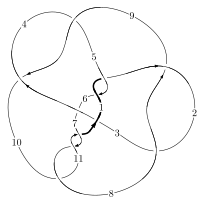
\includegraphics[width=112pt]{../../../GIT/diagram.site/Diagrams/png/787_11n_171.png}\\
\ \ \ A knot diagram\footnotemark}&
\allowdisplaybreaks
\textbf{Linearized knot diagam} \\
\cline{2-2}
 &
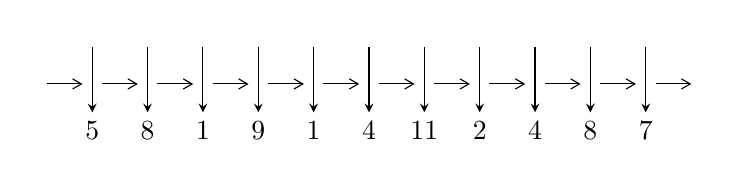
\begin{tikzpicture}[x=20pt, y=17pt]
	% nodes
	\node (C0) at (0, 0) {};
	\node (C1) at (1, 0) {};
	\node (C1U) at (1, +1) {};
	\node (C1D) at (1, -1) {5};

	\node (C2) at (2, 0) {};
	\node (C2U) at (2, +1) {};
	\node (C2D) at (2, -1) {8};

	\node (C3) at (3, 0) {};
	\node (C3U) at (3, +1) {};
	\node (C3D) at (3, -1) {1};

	\node (C4) at (4, 0) {};
	\node (C4U) at (4, +1) {};
	\node (C4D) at (4, -1) {9};

	\node (C5) at (5, 0) {};
	\node (C5U) at (5, +1) {};
	\node (C5D) at (5, -1) {1};

	\node (C6) at (6, 0) {};
	\node (C6U) at (6, +1) {};
	\node (C6D) at (6, -1) {4};

	\node (C7) at (7, 0) {};
	\node (C7U) at (7, +1) {};
	\node (C7D) at (7, -1) {11};

	\node (C8) at (8, 0) {};
	\node (C8U) at (8, +1) {};
	\node (C8D) at (8, -1) {2};

	\node (C9) at (9, 0) {};
	\node (C9U) at (9, +1) {};
	\node (C9D) at (9, -1) {4};

	\node (C10) at (10, 0) {};
	\node (C10U) at (10, +1) {};
	\node (C10D) at (10, -1) {8};

	\node (C11) at (11, 0) {};
	\node (C11U) at (11, +1) {};
	\node (C11D) at (11, -1) {7};
	\node (C12) at (12, 0) {};

	% arrows
	\draw[->,>={angle 60}]
	(C0) edge (C1) (C1) edge (C2) (C2) edge (C3) (C3) edge (C4) (C4) edge (C5) (C5) edge (C6) (C6) edge (C7) (C7) edge (C8) (C8) edge (C9) (C9) edge (C10) (C10) edge (C11) (C11) edge (C12) ;	\draw[->,>=stealth]
	(C1U) edge (C1D) (C2U) edge (C2D) (C3U) edge (C3D) (C4U) edge (C4D) (C5U) edge (C5D) (C6U) edge (C6D) (C7U) edge (C7D) (C8U) edge (C8D) (C9U) edge (C9D) (C10U) edge (C10D) (C11U) edge (C11D) ;
	\end{tikzpicture} \\
\hhline{~~} \\& 
\textbf{Solving Sequence} \\ \cline{2-2} 
 &
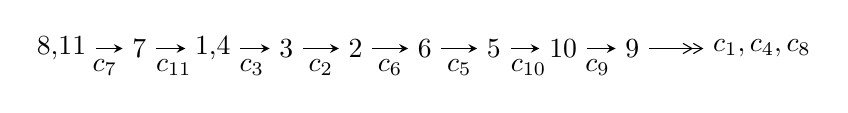
\begin{tikzpicture}[x=25pt, y=7pt]
	% node
	\node (A0) at (-1/8, 0) {8,11};
	\node (A1) at (1, 0) {7};
	\node (A2) at (33/16, 0) {1,4};
	\node (A3) at (25/8, 0) {3};
	\node (A4) at (33/8, 0) {2};
	\node (A5) at (41/8, 0) {6};
	\node (A6) at (49/8, 0) {5};
	\node (A7) at (57/8, 0) {10};
	\node (A8) at (65/8, 0) {9};
	\node (C1) at (1/2, -1) {$c_{7}$};
	\node (C2) at (3/2, -1) {$c_{11}$};
	\node (C3) at (21/8, -1) {$c_{3}$};
	\node (C4) at (29/8, -1) {$c_{2}$};
	\node (C5) at (37/8, -1) {$c_{6}$};
	\node (C6) at (45/8, -1) {$c_{5}$};
	\node (C7) at (53/8, -1) {$c_{10}$};
	\node (C8) at (61/8, -1) {$c_{9}$};
	\node (A9) at (10, 0) {$c_{1},c_{4},c_{8}$};

	% edge
	\draw[->,>=stealth]	
	(A0) edge (A1) (A1) edge (A2) (A2) edge (A3) (A3) edge (A4) (A4) edge (A5) (A5) edge (A6) (A6) edge (A7) (A7) edge (A8) ;
	\draw[->>,>={angle 60}]	
	(A8) edge (A9);
\end{tikzpicture} \\ 

\end{tabular} \\

\footnotetext{
The image of knot diagram is generated by the software ``\textbf{Draw programme}" developed by Andrew Bartholomew(\url{http://www.layer8.co.uk/maths/draw/index.htm\#Running-draw}), where we modified some parts for our purpose(\url{https://github.com/CATsTAILs/LinksPainter}).
}\phantom \\ \newline 
\centering \textbf{Ideals for irreducible components\footnotemark of $X_{\text{par}}$} 
 
\begin{align*}
I^u_{1}&=\langle 
3 u^{16}+14 u^{15}+\cdots+2 b-4,\;u^{16}+5 u^{15}+\cdots+2 a+5,\;u^{17}+6 u^{16}+\cdots-10 u-4\rangle \\
I^u_{2}&=\langle 
38 u^5 a^3-19 u^5 a^2+\cdots+10 a-14,\;-2 u^5 a^2+5 u^5 a+\cdots-9 a+11,\;u^6- u^5+3 u^4-2 u^3+2 u^2- u-1\rangle \\
I^u_{3}&=\langle 
- u^8+u^7-5 u^6+4 u^5-7 u^4+5 u^3-2 u^2+b+3 u,\;- u^8-4 u^6- u^5-3 u^4-3 u^3+3 u^2+a- u+3,\\
\phantom{I^u_{3}}&\phantom{= \langle  }u^9- u^8+6 u^7-5 u^6+12 u^5-8 u^4+8 u^3-5 u^2-1\rangle \\
\\
\end{align*}
\raggedright * 3 irreducible components of $\dim_{\mathbb{C}}=0$, with total 50 representations.\\
\footnotetext{All coefficients of polynomials are rational numbers. But the coefficients are sometimes approximated in decimal forms when there is not enough margin.}
\newpage
\renewcommand{\arraystretch}{1}
\centering \section*{I. $I^u_{1}= \langle 3 u^{16}+14 u^{15}+\cdots+2 b-4,\;u^{16}+5 u^{15}+\cdots+2 a+5,\;u^{17}+6 u^{16}+\cdots-10 u-4 \rangle$}
\flushleft \textbf{(i) Arc colorings}\\
\begin{tabular}{m{7pt} m{180pt} m{7pt} m{180pt} }
\flushright $a_{8}=$&$\begin{pmatrix}1\\0\end{pmatrix}$ \\
\flushright $a_{11}=$&$\begin{pmatrix}0\\u\end{pmatrix}$ \\
\flushright $a_{7}=$&$\begin{pmatrix}1\\- u^2\end{pmatrix}$ \\
\flushright $a_{1}=$&$\begin{pmatrix}- u\\u^3+u\end{pmatrix}$ \\
\flushright $a_{4}=$&$\begin{pmatrix}-\frac{1}{2} u^{16}-\frac{5}{2} u^{15}+\cdots+u-\frac{5}{2}\\-\frac{3}{2} u^{16}-7 u^{15}+\cdots+\frac{11}{2} u+2\end{pmatrix}$ \\
\flushright $a_{3}=$&$\begin{pmatrix}-\frac{1}{2} u^{16}-\frac{3}{2} u^{15}+\cdots+2 u-\frac{1}{2}\\\frac{3}{2} u^{16}+7 u^{15}+\cdots-\frac{11}{2} u-4\end{pmatrix}$ \\
\flushright $a_{2}=$&$\begin{pmatrix}u^{16}+\frac{11}{2} u^{15}+\cdots-\frac{7}{2} u-\frac{9}{2}\\\frac{3}{2} u^{16}+7 u^{15}+\cdots-\frac{11}{2} u-4\end{pmatrix}$ \\
\flushright $a_{6}=$&$\begin{pmatrix}\frac{3}{4} u^{16}+4 u^{15}+\cdots-\frac{15}{4} u-3\\\frac{1}{2} u^{16}+3 u^{15}+\cdots-\frac{3}{2} u-3\end{pmatrix}$ \\
\flushright $a_{5}=$&$\begin{pmatrix}\frac{3}{4} u^{16}+4 u^{15}+\cdots-\frac{15}{4} u-5\\\frac{1}{2} u^{16}+2 u^{15}+\cdots-\frac{3}{2} u-1\end{pmatrix}$ \\
\flushright $a_{10}=$&$\begin{pmatrix}u\\u\end{pmatrix}$ \\
\flushright $a_{9}=$&$\begin{pmatrix}-\frac{1}{4} u^{16}- u^{15}+\cdots+\frac{11}{4} u^2+\frac{1}{4} u\\\frac{1}{2} u^{16}+3 u^{15}+\cdots-\frac{9}{2} u-3\end{pmatrix}$\\ \flushright $a_{9}=$&$\begin{pmatrix}-\frac{1}{4} u^{16}- u^{15}+\cdots+\frac{11}{4} u^2+\frac{1}{4} u\\\frac{1}{2} u^{16}+3 u^{15}+\cdots-\frac{9}{2} u-3\end{pmatrix}$\\&\end{tabular}
\flushleft \textbf{(ii) Obstruction class $= -1$}\\~\\
\flushleft \textbf{(iii) Cusp Shapes $= 4 u^{16}+21 u^{15}+86 u^{14}+243 u^{13}+565 u^{12}+1065 u^{11}+1695 u^{10}+2282 u^9+2614 u^8+2548 u^7+2087 u^6+1403 u^5+739 u^4+258 u^3+31 u^2-30 u-26$}\\~\\
\newpage\renewcommand{\arraystretch}{1}
\flushleft \textbf{(iv) u-Polynomials at the component}\newline \\
\begin{tabular}{m{50pt}|m{274pt}}
Crossings & \hspace{64pt}u-Polynomials at each crossing \\
\hline $$\begin{aligned}c_{1},c_{5}\end{aligned}$$&$\begin{aligned}
&u^{17}+13 u^{16}+\cdots+608 u+64
\end{aligned}$\\
\hline $$\begin{aligned}c_{2},c_{4},c_{8}\\c_{9}\end{aligned}$$&$\begin{aligned}
&u^{17}+5 u^{15}+\cdots+2 u+1
\end{aligned}$\\
\hline $$\begin{aligned}c_{3},c_{6}\end{aligned}$$&$\begin{aligned}
&u^{17}- u^{16}+\cdots-2 u+1
\end{aligned}$\\
\hline $$\begin{aligned}c_{7},c_{10},c_{11}\end{aligned}$$&$\begin{aligned}
&u^{17}-6 u^{16}+\cdots-10 u+4
\end{aligned}$\\
\hline
\end{tabular}\\~\\
\newpage\renewcommand{\arraystretch}{1}
\flushleft \textbf{(v) Riley Polynomials at the component}\newline \\
\begin{tabular}{m{50pt}|m{274pt}}
Crossings & \hspace{64pt}Riley Polynomials at each crossing \\
\hline $$\begin{aligned}c_{1},c_{5}\end{aligned}$$&$\begin{aligned}
&y^{17}+7 y^{16}+\cdots+25600 y-4096
\end{aligned}$\\
\hline $$\begin{aligned}c_{2},c_{4},c_{8}\\c_{9}\end{aligned}$$&$\begin{aligned}
&y^{17}+10 y^{16}+\cdots+2 y-1
\end{aligned}$\\
\hline $$\begin{aligned}c_{3},c_{6}\end{aligned}$$&$\begin{aligned}
&y^{17}-19 y^{16}+\cdots+26 y-1
\end{aligned}$\\
\hline $$\begin{aligned}c_{7},c_{10},c_{11}\end{aligned}$$&$\begin{aligned}
&y^{17}+16 y^{16}+\cdots+172 y-16
\end{aligned}$\\
\hline
\end{tabular}\\~\\
\newpage\flushleft \textbf{(vi) Complex Volumes and Cusp Shapes}
$$\begin{array}{c|c|c}  
\text{Solutions to }I^u_{1}& \I (\text{vol} + \sqrt{-1}CS) & \text{Cusp shape}\\
 \hline 
\begin{aligned}
u &= \phantom{-}0.211807 + 0.989057 I \\
a &= \phantom{-}0.005734 + 0.720235 I \\
b &= \phantom{-}0.595368 + 0.304010 I\end{aligned}
 & \phantom{-}2.01657 - 1.88656 I & -7.16642 + 4.34239 I \\ \hline\begin{aligned}
u &= \phantom{-}0.211807 - 0.989057 I \\
a &= \phantom{-}0.005734 - 0.720235 I \\
b &= \phantom{-}0.595368 - 0.304010 I\end{aligned}
 & \phantom{-}2.01657 + 1.88656 I & -7.16642 - 4.34239 I \\ \hline\begin{aligned}
u &= -0.939675 + 0.221289 I \\
a &= \phantom{-}0.144054 + 0.332191 I \\
b &= \phantom{-}1.160160 - 0.774359 I\end{aligned}
 & -0.01418 + 8.74564 I & -9.43323 - 6.21574 I \\ \hline\begin{aligned}
u &= -0.939675 - 0.221289 I \\
a &= \phantom{-}0.144054 - 0.332191 I \\
b &= \phantom{-}1.160160 + 0.774359 I\end{aligned}
 & -0.01418 - 8.74564 I & -9.43323 + 6.21574 I \\ \hline\begin{aligned}
u &= -0.284641 + 1.111420 I \\
a &= \phantom{-}0.49091 - 1.57082 I \\
b &= \phantom{-}0.271257 - 0.887192 I\end{aligned}
 & -0.64441 + 2.30767 I & -10.18608 - 0.27730 I \\ \hline\begin{aligned}
u &= -0.284641 - 1.111420 I \\
a &= \phantom{-}0.49091 + 1.57082 I \\
b &= \phantom{-}0.271257 + 0.887192 I\end{aligned}
 & -0.64441 - 2.30767 I & -10.18608 + 0.27730 I \\ \hline\begin{aligned}
u &= -0.591453 + 1.005910 I \\
a &= -0.743115 + 0.715842 I \\
b &= -0.247326 - 0.243911 I\end{aligned}
 & \phantom{-}2.42082 - 3.43267 I & -8.02158 + 2.98804 I \\ \hline\begin{aligned}
u &= -0.591453 - 1.005910 I \\
a &= -0.743115 - 0.715842 I \\
b &= -0.247326 + 0.243911 I\end{aligned}
 & \phantom{-}2.42082 + 3.43267 I & -8.02158 - 2.98804 I \\ \hline\begin{aligned}
u &= -0.741532 + 0.257409 I \\
a &= -0.268555 - 0.609503 I \\
b &= -1.069590 + 0.137343 I\end{aligned}
 & -3.15113 + 1.41738 I & -9.71131 - 4.88398 I \\ \hline\begin{aligned}
u &= -0.741532 - 0.257409 I \\
a &= -0.268555 + 0.609503 I \\
b &= -1.069590 - 0.137343 I\end{aligned}
 & -3.15113 - 1.41738 I & -9.71131 + 4.88398 I\\
 \hline 
 \end{array}$$\newpage$$\begin{array}{c|c|c}  
\text{Solutions to }I^u_{1}& \I (\text{vol} + \sqrt{-1}CS) & \text{Cusp shape}\\
 \hline 
\begin{aligned}
u &= -0.41260 + 1.41870 I \\
a &= -0.57836 + 1.72237 I \\
b &= -1.61137 + 1.55108 I\end{aligned}
 & \phantom{-}5.1608 + 13.6066 I & -5.59446 - 7.46007 I \\ \hline\begin{aligned}
u &= -0.41260 - 1.41870 I \\
a &= -0.57836 - 1.72237 I \\
b &= -1.61137 - 1.55108 I\end{aligned}
 & \phantom{-}5.1608 - 13.6066 I & -5.59446 + 7.46007 I \\ \hline\begin{aligned}
u &= -0.32482 + 1.45291 I \\
a &= \phantom{-}0.99147 - 1.18539 I \\
b &= \phantom{-}1.70555 - 1.12903 I\end{aligned}
 & \phantom{-}2.38666 + 5.36037 I & -5.12085 - 4.62281 I \\ \hline\begin{aligned}
u &= -0.32482 - 1.45291 I \\
a &= \phantom{-}0.99147 + 1.18539 I \\
b &= \phantom{-}1.70555 + 1.12903 I\end{aligned}
 & \phantom{-}2.38666 - 5.36037 I & -5.12085 + 4.62281 I \\ \hline\begin{aligned}
u &= -0.05895 + 1.66246 I \\
a &= -0.577246 + 0.085860 I \\
b &= -1.142700 + 0.323103 I\end{aligned}
 & \phantom{-}11.85540 - 1.51678 I & -9.69360 + 5.86030 I \\ \hline\begin{aligned}
u &= -0.05895 - 1.66246 I \\
a &= -0.577246 - 0.085860 I \\
b &= -1.142700 - 0.323103 I\end{aligned}
 & \phantom{-}11.85540 + 1.51678 I & -9.69360 - 5.86030 I \\ \hline\begin{aligned}
u &= \phantom{-}0.283727\phantom{ +0.000000I} \\
a &= \phantom{-}1.07024\phantom{ +0.000000I} \\
b &= -0.322697\phantom{ +0.000000I}\end{aligned}
 & -0.582703\phantom{ +0.000000I} & -17.1450\phantom{ +0.000000I}\\
 \hline 
 \end{array}$$\newpage\newpage\renewcommand{\arraystretch}{1}
\centering \section*{II. $I^u_{2}= \langle 38 u^5 a^3-19 u^5 a^2+\cdots+10 a-14,\;-2 u^5 a^2+5 u^5 a+\cdots-9 a+11,\;u^6- u^5+3 u^4-2 u^3+2 u^2- u-1 \rangle$}
\flushleft \textbf{(i) Arc colorings}\\
\begin{tabular}{m{7pt} m{180pt} m{7pt} m{180pt} }
\flushright $a_{8}=$&$\begin{pmatrix}1\\0\end{pmatrix}$ \\
\flushright $a_{11}=$&$\begin{pmatrix}0\\u\end{pmatrix}$ \\
\flushright $a_{7}=$&$\begin{pmatrix}1\\- u^2\end{pmatrix}$ \\
\flushright $a_{1}=$&$\begin{pmatrix}- u\\u^3+u\end{pmatrix}$ \\
\flushright $a_{4}=$&$\begin{pmatrix}a\\-4.22222 a^{3} u^{5}+2.11111 a^{2} u^{5}+\cdots-1.11111 a+1.55556\end{pmatrix}$ \\
\flushright $a_{3}=$&$\begin{pmatrix}-3.22222 a^{3} u^{5}+2.11111 a^{2} u^{5}+\cdots-0.111111 a-0.444444\\\frac{11}{9} u^5 a^3-\frac{10}{9} u^5 a^2+\cdots+\frac{1}{9} a+\frac{13}{9}\end{pmatrix}$ \\
\flushright $a_{2}=$&$\begin{pmatrix}-2 u^5 a^3+u^5 a^2+\cdots+a^2+1\\\frac{11}{9} u^5 a^3-\frac{10}{9} u^5 a^2+\cdots+\frac{1}{9} a+\frac{13}{9}\end{pmatrix}$ \\
\flushright $a_{6}=$&$\begin{pmatrix}\frac{8}{9} u^5 a^3-\frac{8}{9} u^5 a^2+\cdots+\frac{13}{9} a-\frac{4}{9}\\\frac{8}{9} u^5 a^2-\frac{4}{9} u^5+\cdots+\frac{10}{9} a^2+\frac{4}{9}\end{pmatrix}$ \\
\flushright $a_{5}=$&$\begin{pmatrix}\frac{5}{3} u^5 a^3-\frac{16}{9} u^5 a^2+\cdots+\frac{7}{3} a-\frac{8}{9}\\-\frac{23}{9} u^5 a^3+\frac{5}{3} u^5 a^2+\cdots-\frac{7}{9} a+\frac{4}{3}\end{pmatrix}$ \\
\flushright $a_{10}=$&$\begin{pmatrix}u\\u\end{pmatrix}$ \\
\flushright $a_{9}=$&$\begin{pmatrix}\frac{10}{9} u^5 a^3-\frac{10}{9} u^5 a^2+\cdots-\frac{4}{9} a+\frac{4}{9}\\-1.22222 a^{3} u^{5}+2.33333 a^{2} u^{5}+\cdots-1.11111 a-1.33333\end{pmatrix}$\\ \flushright $a_{9}=$&$\begin{pmatrix}\frac{10}{9} u^5 a^3-\frac{10}{9} u^5 a^2+\cdots-\frac{4}{9} a+\frac{4}{9}\\-1.22222 a^{3} u^{5}+2.33333 a^{2} u^{5}+\cdots-1.11111 a-1.33333\end{pmatrix}$\\&\end{tabular}
\flushleft \textbf{(ii) Obstruction class $= -1$}\\~\\
\flushleft \textbf{(iii) Cusp Shapes $= -\frac{44}{9} u^5 a^3+\frac{40}{9} u^5 a^2+\cdots-\frac{40}{9} a-\frac{106}{9}$}\\~\\
\newpage\renewcommand{\arraystretch}{1}
\flushleft \textbf{(iv) u-Polynomials at the component}\newline \\
\begin{tabular}{m{50pt}|m{274pt}}
Crossings & \hspace{64pt}u-Polynomials at each crossing \\
\hline $$\begin{aligned}c_{1},c_{5}\end{aligned}$$&$\begin{aligned}
&(u^2- u+1)^{12}
\end{aligned}$\\
\hline $$\begin{aligned}c_{2},c_{4},c_{8}\\c_{9}\end{aligned}$$&$\begin{aligned}
&u^{24}- u^{23}+\cdots-26 u+79
\end{aligned}$\\
\hline $$\begin{aligned}c_{3},c_{6}\end{aligned}$$&$\begin{aligned}
&u^{24}-5 u^{23}+\cdots+36 u+13
\end{aligned}$\\
\hline $$\begin{aligned}c_{7},c_{10},c_{11}\end{aligned}$$&$\begin{aligned}
&(u^6+u^5+3 u^4+2 u^3+2 u^2+u-1)^4
\end{aligned}$\\
\hline
\end{tabular}\\~\\
\newpage\renewcommand{\arraystretch}{1}
\flushleft \textbf{(v) Riley Polynomials at the component}\newline \\
\begin{tabular}{m{50pt}|m{274pt}}
Crossings & \hspace{64pt}Riley Polynomials at each crossing \\
\hline $$\begin{aligned}c_{1},c_{5}\end{aligned}$$&$\begin{aligned}
&(y^2+y+1)^{12}
\end{aligned}$\\
\hline $$\begin{aligned}c_{2},c_{4},c_{8}\\c_{9}\end{aligned}$$&$\begin{aligned}
&y^{24}+15 y^{23}+\cdots+53676 y+6241
\end{aligned}$\\
\hline $$\begin{aligned}c_{3},c_{6}\end{aligned}$$&$\begin{aligned}
&y^{24}-5 y^{23}+\cdots-5352 y+169
\end{aligned}$\\
\hline $$\begin{aligned}c_{7},c_{10},c_{11}\end{aligned}$$&$\begin{aligned}
&(y^6+5 y^5+9 y^4+4 y^3-6 y^2-5 y+1)^4
\end{aligned}$\\
\hline
\end{tabular}\\~\\
\newpage\flushleft \textbf{(vi) Complex Volumes and Cusp Shapes}
$$\begin{array}{c|c|c}  
\text{Solutions to }I^u_{2}& \I (\text{vol} + \sqrt{-1}CS) & \text{Cusp shape}\\
 \hline 
\begin{aligned}
u &= \phantom{-}0.873214\phantom{ +0.000000I} \\
a &= \phantom{-}0.374038 + 0.292431 I \\
b &= \phantom{-}0.837071 - 0.727051 I\end{aligned}
 & -2.72528 + 2.02988 I & -10.26950 - 3.46410 I \\ \hline\begin{aligned}
u &= \phantom{-}0.873214\phantom{ +0.000000I} \\
a &= \phantom{-}0.374038 - 0.292431 I \\
b &= \phantom{-}0.837071 + 0.727051 I\end{aligned}
 & -2.72528 - 2.02988 I & -10.26950 + 3.46410 I \\ \hline\begin{aligned}
u &= \phantom{-}0.873214\phantom{ +0.000000I} \\
a &= \phantom{-}0.021379 + 0.392452 I \\
b &= -1.322910 - 0.114439 I\end{aligned}
 & -2.72528 + 2.02988 I & -10.26950 - 3.46410 I \\ \hline\begin{aligned}
u &= \phantom{-}0.873214\phantom{ +0.000000I} \\
a &= \phantom{-}0.021379 - 0.392452 I \\
b &= -1.322910 + 0.114439 I\end{aligned}
 & -2.72528 - 2.02988 I & -10.26950 + 3.46410 I \\ \hline\begin{aligned}
u &= -0.138835 + 1.234450 I \\
a &= -0.541688 + 0.032957 I \\
b &= \phantom{-}0.769169 - 0.336322 I\end{aligned}
 & \phantom{-}7.89505 - 0.05747 I & -2.57572 - 0.22068 I \\ \hline\begin{aligned}
u &= -0.138835 + 1.234450 I \\
a &= -1.30626 + 0.70357 I \\
b &= -2.42790 + 0.70593 I\end{aligned}
 & \phantom{-}7.89505 + 4.00229 I & -2.57572 - 7.14888 I \\ \hline\begin{aligned}
u &= -0.138835 + 1.234450 I \\
a &= -0.86980 - 2.16519 I \\
b &= \phantom{-}0.20728 - 1.55918 I\end{aligned}
 & \phantom{-}7.89505 + 4.00229 I & -2.57572 - 7.14888 I \\ \hline\begin{aligned}
u &= -0.138835 + 1.234450 I \\
a &= \phantom{-}0.36392 + 2.58238 I \\
b &= -0.39780 + 2.68606 I\end{aligned}
 & \phantom{-}7.89505 - 0.05747 I & -2.57572 - 0.22068 I \\ \hline\begin{aligned}
u &= -0.138835 - 1.234450 I \\
a &= -0.541688 - 0.032957 I \\
b &= \phantom{-}0.769169 + 0.336322 I\end{aligned}
 & \phantom{-}7.89505 + 0.05747 I & -2.57572 + 0.22068 I \\ \hline\begin{aligned}
u &= -0.138835 - 1.234450 I \\
a &= -1.30626 - 0.70357 I \\
b &= -2.42790 - 0.70593 I\end{aligned}
 & \phantom{-}7.89505 - 4.00229 I & -2.57572 + 7.14888 I\\
 \hline 
 \end{array}$$\newpage$$\begin{array}{c|c|c}  
\text{Solutions to }I^u_{2}& \I (\text{vol} + \sqrt{-1}CS) & \text{Cusp shape}\\
 \hline 
\begin{aligned}
u &= -0.138835 - 1.234450 I \\
a &= -0.86980 + 2.16519 I \\
b &= \phantom{-}0.20728 + 1.55918 I\end{aligned}
 & \phantom{-}7.89505 - 4.00229 I & -2.57572 + 7.14888 I \\ \hline\begin{aligned}
u &= -0.138835 - 1.234450 I \\
a &= \phantom{-}0.36392 - 2.58238 I \\
b &= -0.39780 - 2.68606 I\end{aligned}
 & \phantom{-}7.89505 + 0.05747 I & -2.57572 + 0.22068 I \\ \hline\begin{aligned}
u &= \phantom{-}0.408802 + 1.276380 I \\
a &= -0.605131 - 0.405910 I \\
b &= -0.216543 - 0.031148 I\end{aligned}
 & \phantom{-}1.23922 - 2.56224 I & -6.58114 - 0.25928 I \\ \hline\begin{aligned}
u &= \phantom{-}0.408802 + 1.276380 I \\
a &= \phantom{-}0.606056 + 1.218440 I \\
b &= \phantom{-}1.35224 + 0.72201 I\end{aligned}
 & \phantom{-}1.23922 - 2.56224 I & -6.58114 - 0.25928 I \\ \hline\begin{aligned}
u &= \phantom{-}0.408802 + 1.276380 I \\
a &= \phantom{-}0.76345 + 1.35547 I \\
b &= \phantom{-}0.949823 + 0.357497 I\end{aligned}
 & \phantom{-}1.23922 - 6.62201 I & -6.58114 + 6.66892 I \\ \hline\begin{aligned}
u &= \phantom{-}0.408802 + 1.276380 I \\
a &= -0.06024 - 1.76254 I \\
b &= -0.91937 - 1.68647 I\end{aligned}
 & \phantom{-}1.23922 - 6.62201 I & -6.58114 + 6.66892 I \\ \hline\begin{aligned}
u &= \phantom{-}0.408802 - 1.276380 I \\
a &= -0.605131 + 0.405910 I \\
b &= -0.216543 + 0.031148 I\end{aligned}
 & \phantom{-}1.23922 + 2.56224 I & -6.58114 + 0.25928 I \\ \hline\begin{aligned}
u &= \phantom{-}0.408802 - 1.276380 I \\
a &= \phantom{-}0.606056 - 1.218440 I \\
b &= \phantom{-}1.35224 - 0.72201 I\end{aligned}
 & \phantom{-}1.23922 + 2.56224 I & -6.58114 + 0.25928 I \\ \hline\begin{aligned}
u &= \phantom{-}0.408802 - 1.276380 I \\
a &= \phantom{-}0.76345 - 1.35547 I \\
b &= \phantom{-}0.949823 - 0.357497 I\end{aligned}
 & \phantom{-}1.23922 + 6.62201 I & -6.58114 - 6.66892 I \\ \hline\begin{aligned}
u &= \phantom{-}0.408802 - 1.276380 I \\
a &= -0.06024 + 1.76254 I \\
b &= -0.91937 + 1.68647 I\end{aligned}
 & \phantom{-}1.23922 + 6.62201 I & -6.58114 - 6.66892 I\\
 \hline 
 \end{array}$$\newpage$$\begin{array}{c|c|c}  
\text{Solutions to }I^u_{2}& \I (\text{vol} + \sqrt{-1}CS) & \text{Cusp shape}\\
 \hline 
\begin{aligned}
u &= -0.413150\phantom{ +0.000000I} \\
a &= \phantom{-}1.19455 + 0.88026 I \\
b &= \phantom{-}0.07172 - 1.48991 I\end{aligned}
 & \phantom{-}4.19595 - 2.02988 I & -11.41678 + 3.46410 I \\ \hline\begin{aligned}
u &= -0.413150\phantom{ +0.000000I} \\
a &= \phantom{-}1.19455 - 0.88026 I \\
b &= \phantom{-}0.07172 + 1.48991 I\end{aligned}
 & \phantom{-}4.19595 + 2.02988 I & -11.41678 - 3.46410 I \\ \hline\begin{aligned}
u &= -0.413150\phantom{ +0.000000I} \\
a &= \phantom{-}0.05973 + 3.05273 I \\
b &= \phantom{-}0.597209 - 0.331281 I\end{aligned}
 & \phantom{-}4.19595 + 2.02988 I & -11.41678 - 3.46410 I \\ \hline\begin{aligned}
u &= -0.413150\phantom{ +0.000000I} \\
a &= \phantom{-}0.05973 - 3.05273 I \\
b &= \phantom{-}0.597209 + 0.331281 I\end{aligned}
 & \phantom{-}4.19595 - 2.02988 I & -11.41678 + 3.46410 I\\
 \hline 
 \end{array}$$\newpage\newpage\renewcommand{\arraystretch}{1}
\centering \section*{III. $I^u_{3}= \langle - u^8+u^7+\cdots+b+3 u,\;- u^8-4 u^6- u^5-3 u^4-3 u^3+3 u^2+a- u+3,\;u^9- u^8+\cdots-5 u^2-1 \rangle$}
\flushleft \textbf{(i) Arc colorings}\\
\begin{tabular}{m{7pt} m{180pt} m{7pt} m{180pt} }
\flushright $a_{8}=$&$\begin{pmatrix}1\\0\end{pmatrix}$ \\
\flushright $a_{11}=$&$\begin{pmatrix}0\\u\end{pmatrix}$ \\
\flushright $a_{7}=$&$\begin{pmatrix}1\\- u^2\end{pmatrix}$ \\
\flushright $a_{1}=$&$\begin{pmatrix}- u\\u^3+u\end{pmatrix}$ \\
\flushright $a_{4}=$&$\begin{pmatrix}u^8+4 u^6+u^5+3 u^4+3 u^3-3 u^2+u-3\\u^8- u^7+5 u^6-4 u^5+7 u^4-5 u^3+2 u^2-3 u\end{pmatrix}$ \\
\flushright $a_{3}=$&$\begin{pmatrix}u^7- u^6+5 u^5-4 u^4+7 u^3-5 u^2+2 u-3\\u^8- u^7+5 u^6-4 u^5+8 u^4-5 u^3+4 u^2-3 u\end{pmatrix}$ \\
\flushright $a_{2}=$&$\begin{pmatrix}u^8+4 u^6+u^5+4 u^4+2 u^3- u^2- u-3\\u^8- u^7+5 u^6-4 u^5+8 u^4-5 u^3+4 u^2-3 u\end{pmatrix}$ \\
\flushright $a_{6}=$&$\begin{pmatrix}u^6-2 u^5+5 u^4-7 u^3+7 u^2-5 u+2\\- u^8+2 u^7-6 u^6+8 u^5-11 u^4+8 u^3-6 u^2+u\end{pmatrix}$ \\
\flushright $a_{5}=$&$\begin{pmatrix}- u^7+2 u^6-6 u^5+8 u^4-11 u^3+9 u^2-5 u+2\\- u^8+u^7-5 u^6+4 u^5-8 u^4+4 u^3-3 u^2+u+1\end{pmatrix}$ \\
\flushright $a_{10}=$&$\begin{pmatrix}u\\u\end{pmatrix}$ \\
\flushright $a_{9}=$&$\begin{pmatrix}-2 u^8+3 u^7-12 u^6+14 u^5-23 u^4+19 u^3-13 u^2+8 u\\u^7- u^6+5 u^5-4 u^4+7 u^3-4 u^2+2 u-2\end{pmatrix}$\\ \flushright $a_{9}=$&$\begin{pmatrix}-2 u^8+3 u^7-12 u^6+14 u^5-23 u^4+19 u^3-13 u^2+8 u\\u^7- u^6+5 u^5-4 u^4+7 u^3-4 u^2+2 u-2\end{pmatrix}$\\&\end{tabular}
\flushleft \textbf{(ii) Obstruction class $= 1$}\\~\\
\flushleft \textbf{(iii) Cusp Shapes $= -3 u^6-11 u^4+u^3-10 u^2+u-3$}\\~\\
\newpage\renewcommand{\arraystretch}{1}
\flushleft \textbf{(iv) u-Polynomials at the component}\newline \\
\begin{tabular}{m{50pt}|m{274pt}}
Crossings & \hspace{64pt}u-Polynomials at each crossing \\
\hline $$\begin{aligned}c_{1}\end{aligned}$$&$\begin{aligned}
&u^9+3 u^7-3 u^6+u^5-4 u^4+3 u^3+u-1
\end{aligned}$\\
\hline $$\begin{aligned}c_{2},c_{9}\end{aligned}$$&$\begin{aligned}
&u^9+4 u^7- u^6+6 u^5-2 u^4+3 u^3- u^2+1
\end{aligned}$\\
\hline $$\begin{aligned}c_{3},c_{6}\end{aligned}$$&$\begin{aligned}
&u^9+u^8+3 u^6+4 u^5+u^4+3 u^3+3 u^2+1
\end{aligned}$\\
\hline $$\begin{aligned}c_{4},c_{8}\end{aligned}$$&$\begin{aligned}
&u^9+4 u^7+u^6+6 u^5+2 u^4+3 u^3+u^2-1
\end{aligned}$\\
\hline $$\begin{aligned}c_{5}\end{aligned}$$&$\begin{aligned}
&u^9+3 u^7+3 u^6+u^5+4 u^4+3 u^3+u+1
\end{aligned}$\\
\hline $$\begin{aligned}c_{7}\end{aligned}$$&$\begin{aligned}
&u^9- u^8+6 u^7-5 u^6+12 u^5-8 u^4+8 u^3-5 u^2-1
\end{aligned}$\\
\hline $$\begin{aligned}c_{10},c_{11}\end{aligned}$$&$\begin{aligned}
&u^9+u^8+6 u^7+5 u^6+12 u^5+8 u^4+8 u^3+5 u^2+1
\end{aligned}$\\
\hline
\end{tabular}\\~\\
\newpage\renewcommand{\arraystretch}{1}
\flushleft \textbf{(v) Riley Polynomials at the component}\newline \\
\begin{tabular}{m{50pt}|m{274pt}}
Crossings & \hspace{64pt}Riley Polynomials at each crossing \\
\hline $$\begin{aligned}c_{1},c_{5}\end{aligned}$$&$\begin{aligned}
&y^9+6 y^8+11 y^7+3 y^6-3 y^5-4 y^4+5 y^3-2 y^2+y-1
\end{aligned}$\\
\hline $$\begin{aligned}c_{2},c_{4},c_{8}\\c_{9}\end{aligned}$$&$\begin{aligned}
&y^9+8 y^8+28 y^7+53 y^6+56 y^5+30 y^4+7 y^3+3 y^2+2 y-1
\end{aligned}$\\
\hline $$\begin{aligned}c_{3},c_{6}\end{aligned}$$&$\begin{aligned}
&y^9- y^8+2 y^7-5 y^6+4 y^5+3 y^4-3 y^3-11 y^2-6 y-1
\end{aligned}$\\
\hline $$\begin{aligned}c_{7},c_{10},c_{11}\end{aligned}$$&$\begin{aligned}
&y^9+11 y^8+50 y^7+119 y^6+150 y^5+76 y^4-26 y^3-41 y^2-10 y-1
\end{aligned}$\\
\hline
\end{tabular}\\~\\
\newpage\flushleft \textbf{(vi) Complex Volumes and Cusp Shapes}
$$\begin{array}{c|c|c}  
\text{Solutions to }I^u_{3}& \I (\text{vol} + \sqrt{-1}CS) & \text{Cusp shape}\\
 \hline 
\begin{aligned}
u &= -0.075853 + 1.213420 I \\
a &= \phantom{-}0.03154 - 1.82376 I \\
b &= \phantom{-}1.20483 - 1.57677 I\end{aligned}
 & \phantom{-}7.92625 + 2.61535 I & -2.34637 - 1.10608 I \\ \hline\begin{aligned}
u &= -0.075853 - 1.213420 I \\
a &= \phantom{-}0.03154 + 1.82376 I \\
b &= \phantom{-}1.20483 + 1.57677 I\end{aligned}
 & \phantom{-}7.92625 - 2.61535 I & -2.34637 + 1.10608 I \\ \hline\begin{aligned}
u &= \phantom{-}0.768805\phantom{ +0.000000I} \\
a &= -0.376504\phantom{ +0.000000I} \\
b &= -1.02947\phantom{ +0.000000I}\end{aligned}
 & -3.42422\phantom{ +0.000000I} & -12.1500\phantom{ +0.000000I} \\ \hline\begin{aligned}
u &= \phantom{-}0.369661 + 1.332040 I \\
a &= \phantom{-}0.614696 + 1.165930 I \\
b &= \phantom{-}1.003450 + 0.853584 I\end{aligned}
 & \phantom{-}0.82219 - 4.09909 I & -8.12215 + 4.24227 I \\ \hline\begin{aligned}
u &= \phantom{-}0.369661 - 1.332040 I \\
a &= \phantom{-}0.614696 - 1.165930 I \\
b &= \phantom{-}1.003450 - 0.853584 I\end{aligned}
 & \phantom{-}0.82219 + 4.09909 I & -8.12215 - 4.24227 I \\ \hline\begin{aligned}
u &= -0.140254 + 0.400864 I \\
a &= -2.50540 + 0.68883 I \\
b &= -0.069927 - 1.023240 I\end{aligned}
 & \phantom{-}5.21158 - 1.80390 I & -1.75250 + 1.15156 I \\ \hline\begin{aligned}
u &= -0.140254 - 0.400864 I \\
a &= -2.50540 - 0.68883 I \\
b &= -0.069927 + 1.023240 I\end{aligned}
 & \phantom{-}5.21158 + 1.80390 I & -1.75250 - 1.15156 I \\ \hline\begin{aligned}
u &= -0.03796 + 1.59738 I \\
a &= -0.452577 + 0.521156 I \\
b &= -1.123620 + 0.702862 I\end{aligned}
 & \phantom{-}12.42610 - 1.12659 I & \phantom{-}0.795880 - 0.970083 I \\ \hline\begin{aligned}
u &= -0.03796 - 1.59738 I \\
a &= -0.452577 - 0.521156 I \\
b &= -1.123620 - 0.702862 I\end{aligned}
 & \phantom{-}12.42610 + 1.12659 I & \phantom{-}0.795880 + 0.970083 I\\
 \hline 
 \end{array}$$\newpage
\newpage\renewcommand{\arraystretch}{1}
\centering \section*{ IV. u-Polynomials}
\begin{tabular}{m{50pt}|m{274pt}}
Crossings & \hspace{64pt}u-Polynomials at each crossing \\
\hline $$\begin{aligned}c_{1}\end{aligned}$$&$\begin{aligned}
&(u^2- u+1)^{12}(u^9+3 u^7-3 u^6+u^5-4 u^4+3 u^3+u-1)\\
&\cdot(u^{17}+13 u^{16}+\cdots+608 u+64)
\end{aligned}$\\
\hline $$\begin{aligned}c_{2},c_{9}\end{aligned}$$&$\begin{aligned}
&(u^9+4 u^7+\cdots- u^2+1)(u^{17}+5 u^{15}+\cdots+2 u+1)\\
&\cdot(u^{24}- u^{23}+\cdots-26 u+79)
\end{aligned}$\\
\hline $$\begin{aligned}c_{3},c_{6}\end{aligned}$$&$\begin{aligned}
&(u^9+u^8+\cdots+3 u^2+1)(u^{17}- u^{16}+\cdots-2 u+1)\\
&\cdot(u^{24}-5 u^{23}+\cdots+36 u+13)
\end{aligned}$\\
\hline $$\begin{aligned}c_{4},c_{8}\end{aligned}$$&$\begin{aligned}
&(u^9+4 u^7+\cdots+u^2-1)(u^{17}+5 u^{15}+\cdots+2 u+1)\\
&\cdot(u^{24}- u^{23}+\cdots-26 u+79)
\end{aligned}$\\
\hline $$\begin{aligned}c_{5}\end{aligned}$$&$\begin{aligned}
&(u^2- u+1)^{12}(u^9+3 u^7+3 u^6+u^5+4 u^4+3 u^3+u+1)\\
&\cdot(u^{17}+13 u^{16}+\cdots+608 u+64)
\end{aligned}$\\
\hline $$\begin{aligned}c_{7}\end{aligned}$$&$\begin{aligned}
&(u^6+u^5+3 u^4+2 u^3+2 u^2+u-1)^4\\
&\cdot(u^9- u^8+6 u^7-5 u^6+12 u^5-8 u^4+8 u^3-5 u^2-1)\\
&\cdot(u^{17}-6 u^{16}+\cdots-10 u+4)
\end{aligned}$\\
\hline $$\begin{aligned}c_{10},c_{11}\end{aligned}$$&$\begin{aligned}
&(u^6+u^5+3 u^4+2 u^3+2 u^2+u-1)^4\\
&\cdot(u^9+u^8+6 u^7+5 u^6+12 u^5+8 u^4+8 u^3+5 u^2+1)\\
&\cdot(u^{17}-6 u^{16}+\cdots-10 u+4)
\end{aligned}$\\
\hline
\end{tabular}\newpage\renewcommand{\arraystretch}{1}
\centering \section*{ V. Riley Polynomials}
\begin{tabular}{m{50pt}|m{274pt}}
Crossings & \hspace{64pt}Riley Polynomials at each crossing \\
\hline $$\begin{aligned}c_{1},c_{5}\end{aligned}$$&$\begin{aligned}
&((y^2+y+1)^{12})(y^9+6 y^8+\cdots+y-1)\\
&\cdot(y^{17}+7 y^{16}+\cdots+25600 y-4096)
\end{aligned}$\\
\hline $$\begin{aligned}c_{2},c_{4},c_{8}\\c_{9}\end{aligned}$$&$\begin{aligned}
&(y^9+8 y^8+28 y^7+53 y^6+56 y^5+30 y^4+7 y^3+3 y^2+2 y-1)\\
&\cdot(y^{17}+10 y^{16}+\cdots+2 y-1)(y^{24}+15 y^{23}+\cdots+53676 y+6241)
\end{aligned}$\\
\hline $$\begin{aligned}c_{3},c_{6}\end{aligned}$$&$\begin{aligned}
&(y^9- y^8+2 y^7-5 y^6+4 y^5+3 y^4-3 y^3-11 y^2-6 y-1)\\
&\cdot(y^{17}-19 y^{16}+\cdots+26 y-1)(y^{24}-5 y^{23}+\cdots-5352 y+169)
\end{aligned}$\\
\hline $$\begin{aligned}c_{7},c_{10},c_{11}\end{aligned}$$&$\begin{aligned}
&(y^6+5 y^5+9 y^4+4 y^3-6 y^2-5 y+1)^4\\
&\cdot(y^9+11 y^8+50 y^7+119 y^6+150 y^5+76 y^4-26 y^3-41 y^2-10 y-1)\\
&\cdot(y^{17}+16 y^{16}+\cdots+172 y-16)
\end{aligned}$\\
\hline
\end{tabular}
\vskip 2pc
\end{document}